\SetPicSubDir{ch-Rice}
\SetExpSubDir{ch-Rice}

\chapter{Experimental Results and Analysis}
\label{ch:rice}
\vspace{2em}

\section{Overview of Experimental Setup}
\subsection{Dataset: Binary MNIST}
The experiment setup utilises a filtered version of the Modified National Institute of Standards and Technology (MNIST) dataset, retaining only samples labelled as digits '0' and '1'. This binarisation process was intentionally designed to simplify the data distribution while preserving sufficient visual complexity for the evaluation of generative performance of GAN models. To address the class imbalance, undersampling was performed for both classes, where samples were randomly selected from the majority class until data counts for both classes matched. This is done to avoid mode collapse and ensure fairness of the experiment. Each image is of dimension $28 \times 28$ pixels and reshaped into a 784-dimensional vector prior to GAN training. All pixel values were also normalised to the range $[-1, 1]$ using the following formula:
\begin{equation}
x_{\text{norm}} = \frac{x - \min}{\max - \min} \times 2 - 1
\end{equation}

Normalisation ensures compatibility with the tanh output activation of the generator. The resulting dataset was then shuffled and batched with a batch size of 64. The usage of the MNIST dataset allows for clearer evaluation of generative performance under noise in quantum circuits, and ensures comparative studies between classical and HQCGAN remains interpretable and computationally tractable.

\subsection{Model Architectures}

The classical GAN implemented in this experiment adopts a fully connected feedforward architecture for both the generator and the discriminator, ideal for flattened binary MNIST dataset of shape $28 \times 28 = 784$. The classical GAN will serve as a basis for the evaluation (baseline) of the HQCGAN in this experiment.

The generator takes a latent input vector \( z \in \mathbb{R}^{100} \), sampled from a standard normal distribution. Subsequently, it passes through two hidden layers with ReLU activation, followed by a final layer with tanh activation to produce an output image vector \( \hat{x} \in \mathbb{R}^{784} \) in the range $[-1, 1]$. The forward pass formula is defined as follows:
\begin{equation}
G(z) = \tanh(W_3 \cdot \text{ReLU}(W_2 \cdot \text{ReLU}(W_1 \cdot z + b_1) + b_2) + b_3)
\end{equation}

The discriminator receives real or generated images and outputs a probability score. It consists of two hidden layers with LeakyReLU activation and a final sigmoid-activated output.

The GAN is trained using the standard non-saturating loss formulation with Binary Cross-Entropy (BCE) as the objective function. The discriminator loss formula is defined as follows:

\begin{equation}
\mathcal{L}_D = -\frac{1}{2} \left[\log D(x) + \log \left(1 - D(G(z))\right)\right]
\end{equation}

The generator loss formula is defined as follows:

\begin{equation}
\mathcal{L}_G = -\log D(G(z))
\end{equation}

These formulas are consistent across all GANs throughout the experiment, with architectural modifications being the only applied changes made for the HQCGAN.
\newpage
\subsection{GAN Variants}

To evaluate the theoretical promises of HQCGAN, we implemented an HQCGAN and a Classical GAN to compare their performance. A summary of the configuration of each model is provided below:

\begin{center}
\begin{tabular}{|c|c|c|c|c|}
\hline
\textbf{Model} & \textbf{Generator Type} & \textbf{Discriminator Type} & \textbf{Latent Dim} & \textbf{Qubits Used} \\
\hline
Classical & Classical & Classical & 100 & 0 \\
HQCGAN-3    & Quantum   & Classical & 3   & 3 \\
HQCGAN-5    & Quantum   & Classical & 5   & 5 \\
HQCGAN-7    & Quantum   & Classical & 7   & 7 \\
\hline
\end{tabular}
\end{center}

\subsection{Quantum Latent Sampling with Noise}

In HQCGAN, the latent vector ($z$) is not sampled from a traditional Gaussian distribution. Instead, it is derived from measurements of noisy quantum circuits simulated using the Qiskit AerSimulator. Each circuit consists of Hadamard Gates applied to all qubits. The resulting bitstrings will be interpreted as binary vectors and linearly scaled to the range $[-1, 1]$ using the following transformation:
\begin{equation}
z = 2 \cdot \text{bitstring\_sample} - 1
\end{equation}
To introduce realistic quantum effects, the circuits were executed on an AerSimulator backend with a custom noise model, incorporating the following: 
\begin{itemize}
\item Depolarising noise: simulates random Pauli errors on gates
\item Amplitude damping: emulates energy relaxation ($T_1$ decay)
\item Readout error: models inaccuracies in measurement outcomes
\end{itemize}
To validate the effect of quantum noise, the state density matrix $\rho$ was extracted and visualised using Qiskit tools in Section 3.2, including:
\begin{itemize}
\item Cityscape plots to visualise real and imaginary components of $\rho$
\item Pauli vector representations to capture expectation values of Pauli observables
\item Bloch multivector diagrams for multi-qubit state structure
\end{itemize}

\subsection{Training Strategy and Metrics}

The training procedure followed the standard GAN loop, with both classical and HQCGAN optimised using the Adam optimiser. Key hyperparameters and metrics tracked throughout the training are detailed below:

\subsubsection{Hyperparameters}

The training of the GAN models was conducted using a batch size of 64 and run over 150 epochs to ensure sufficient exposure to the dataset. The optimiser selected was Adam, a widely used adaptive learning rate optimisation algorithm in deep learning. A learning rate of $0.0002$ was applied, which balances the need for stable convergence with the flexibility to escape local minima. This configuration reflects common best practices for training GANs on datasets of similar size and complexity.

\subsubsection{Accuracy Metrics}

To assess the quality and diversity of the generated images, two key accuracy metrics were used: the Fréchet Inception Distance (FID) and the Kernel Inception Distance (KID). The FID score is defined mathematically as:

\begin{equation}
\text{FID} = \lVert \mu_r - \mu_g \rVert^2 + \text{Tr} \left( \Sigma_r + \Sigma_g - 2 (\Sigma_r \Sigma_g)^{\frac{1}{2}} \right)
\end{equation}

This metric evaluates the distance between the feature distributions of real and generated images, assuming that both follow a multivariate Gaussian distribution. Lower FID values indicate greater similarity between the generated and real data distributions, signifying better visual fidelity and diversity.

On the other hand, the KID is formulated as:

\begin{equation}
\text{KID} = \left\lVert \frac{1}{m} \sum_{i=1}^{m} \phi(x_i) - \frac{1}{n} \sum_{j=1}^{n} \phi(y_j) \right\rVert^2
\end{equation}

Unlike FID, KID uses the Maximum Mean Discrepancy (MMD) with polynomial kernels and does not assume Gaussianity. This makes it particularly suitable for smaller datasets, offering an unbiased estimate of the similarity between real and generated feature representations.

\subsubsection{Efficiency Metrics}

In addition to accuracy, training efficiency was tracked using two practical metrics. The first is the \textbf{time per epoch}, which captures how long it takes the model to complete a single pass through the dataset; this is especially critical when comparing model architectures or performing hyperparameter tuning. The second is the \textbf{total number of samples seen} during training, which provides insight into the scale of data exposure and can help contextualise model convergence patterns and learning stability.

\section{Quantum Circuit Visualisation}

Quantum circuits were used to generate a latent vector ($z$) for the HQCGAN. These circuits were created with the help of the Qiskit AerSimulator, which supports realistic quantum noise modelling. This section presents a visual analysis of the quantum states produced by the circuits used to sample the latent space.

\subsection{Quantum Circuit Diagram}

\begin{figure}[htbp]
\centering
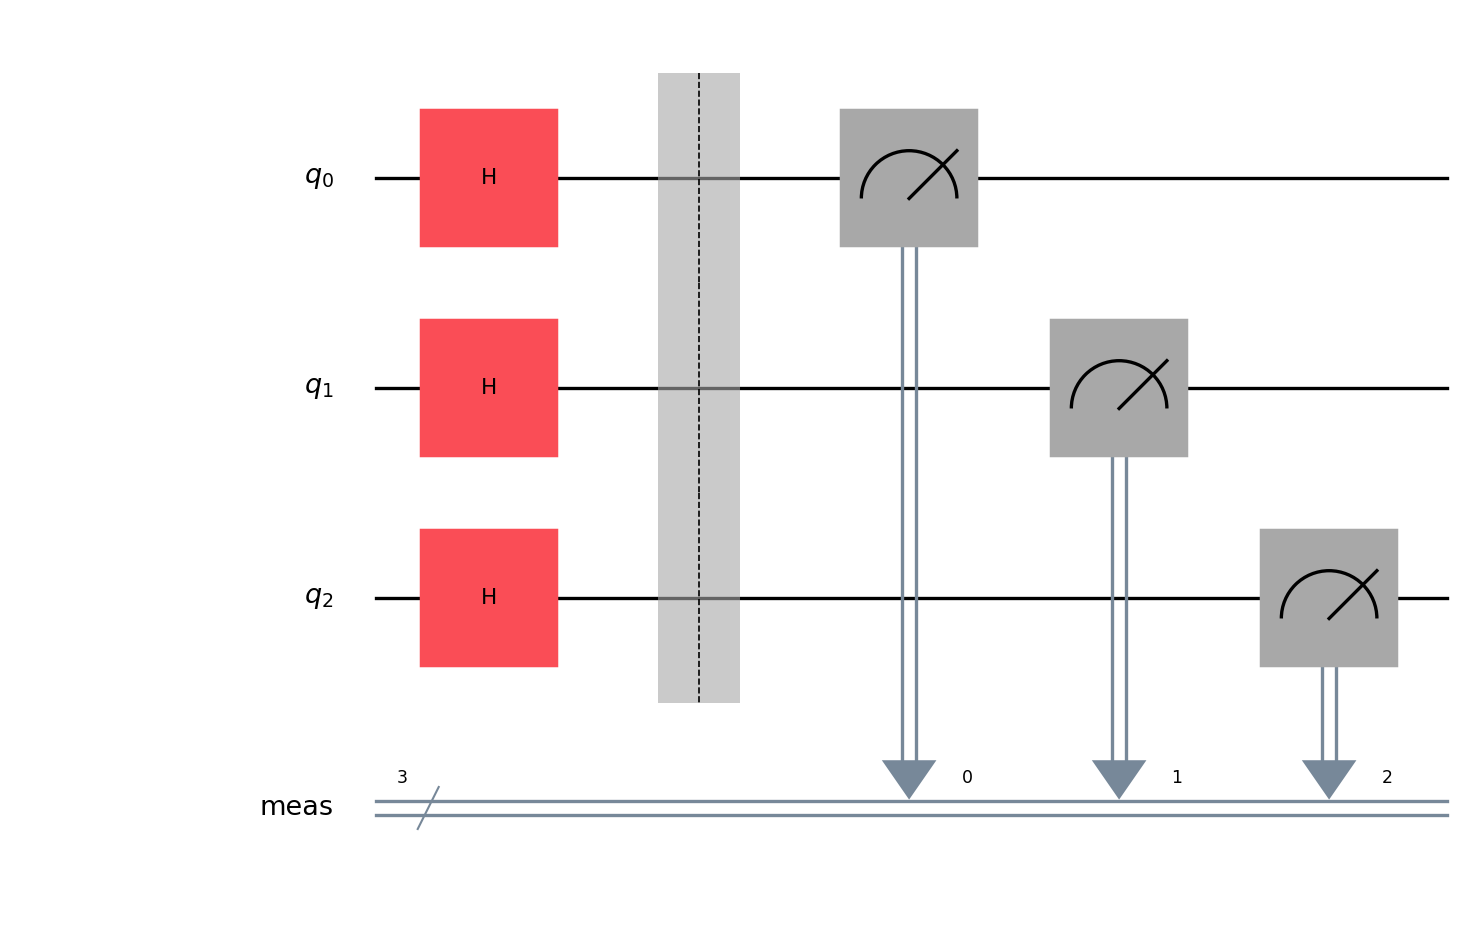
\includegraphics[width=0.75\linewidth]{pic/ch-Rice/QuantumCircuit.png}
\vspace{\BeforeCaptionVSpace}
\caption{Quantum circuit used for sampling latent vectors. Each qubit is initialised in $\left| 0 \right\rangle$ and transformed by Hadamard gates. Full measurement is performed post-noise.}
\label{fig:QuantumCircuit}
\end{figure}

The quantum circuit for each configuration ($n = 3, 5, 7$ qubits) consists of parallel Hadamard Gates, followed by a full measurement. Each qubit is initialised in the $\left| 0 \right\rangle$ state and transformed into a superposition state through the $H$ gate. This will ultimately provide a uniform sampling across all $2^n$ basis states. The quantum circuit is shown in \textbf{Figure~\ref{fig:QuantumCircuit}}.

\subsection{Noisy Density Matrix (Cityscape)}

To understand how quantum noise impacts the state, we visualise the real component of the noisy density matrix as a cityscape plot in \textbf{Figure~\ref{fig:NoisyCityscape}}. This reveals how much of the quantum state remains coherent and decoherent due to the applied noise model.

\begin{figure}[htbp]
\centering
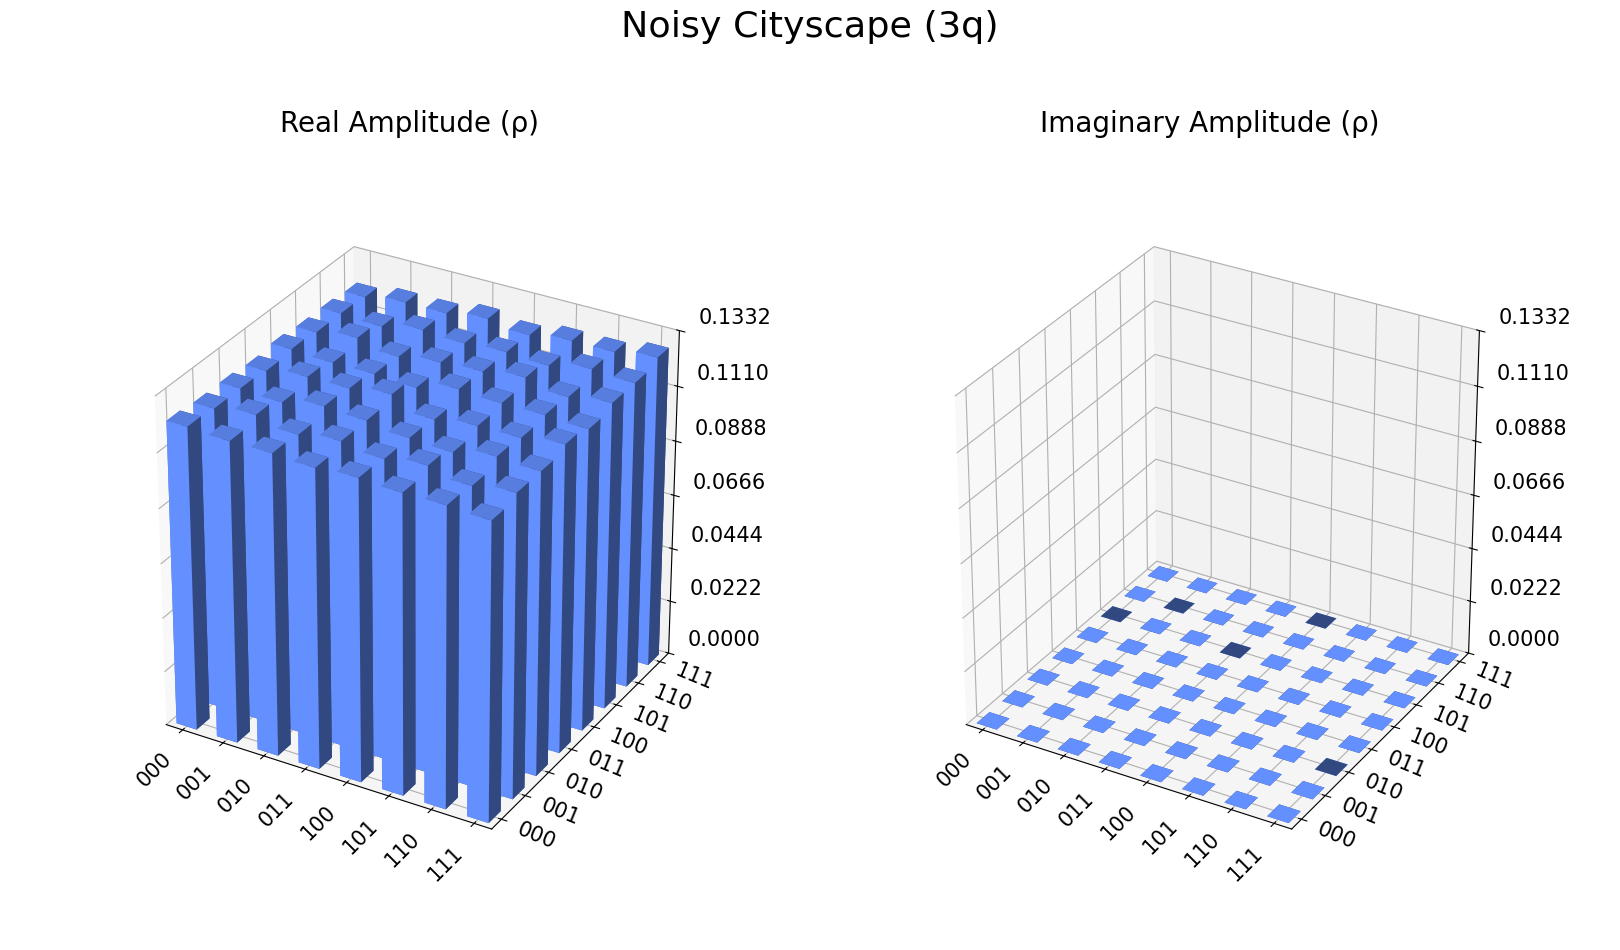
\includegraphics[width=0.75\linewidth]{pic/ch-Rice/NoisyCityScape.png}
\vspace{\BeforeCaptionVSpace}
\caption{Cityscape visualisation of the noisy quantum state density matrix. The z-axis represents the real component of the matrix elements after noise simulation.}
\label{fig:NoisyCityscape}
\end{figure}

\subsection{Pauli Vector Representation}
The Pauli vector visualisation decomposes the quantum state into the basis of Pauli matrices ($I, X, Y, Z$). This is useful to evaluate the amount of remaining coherence and observable noise-induced shrinkage in the Bloch sphere as shown in \textbf{Figure~\ref{fig:PauliVector}}.

\begin{figure}[htbp]
\centering
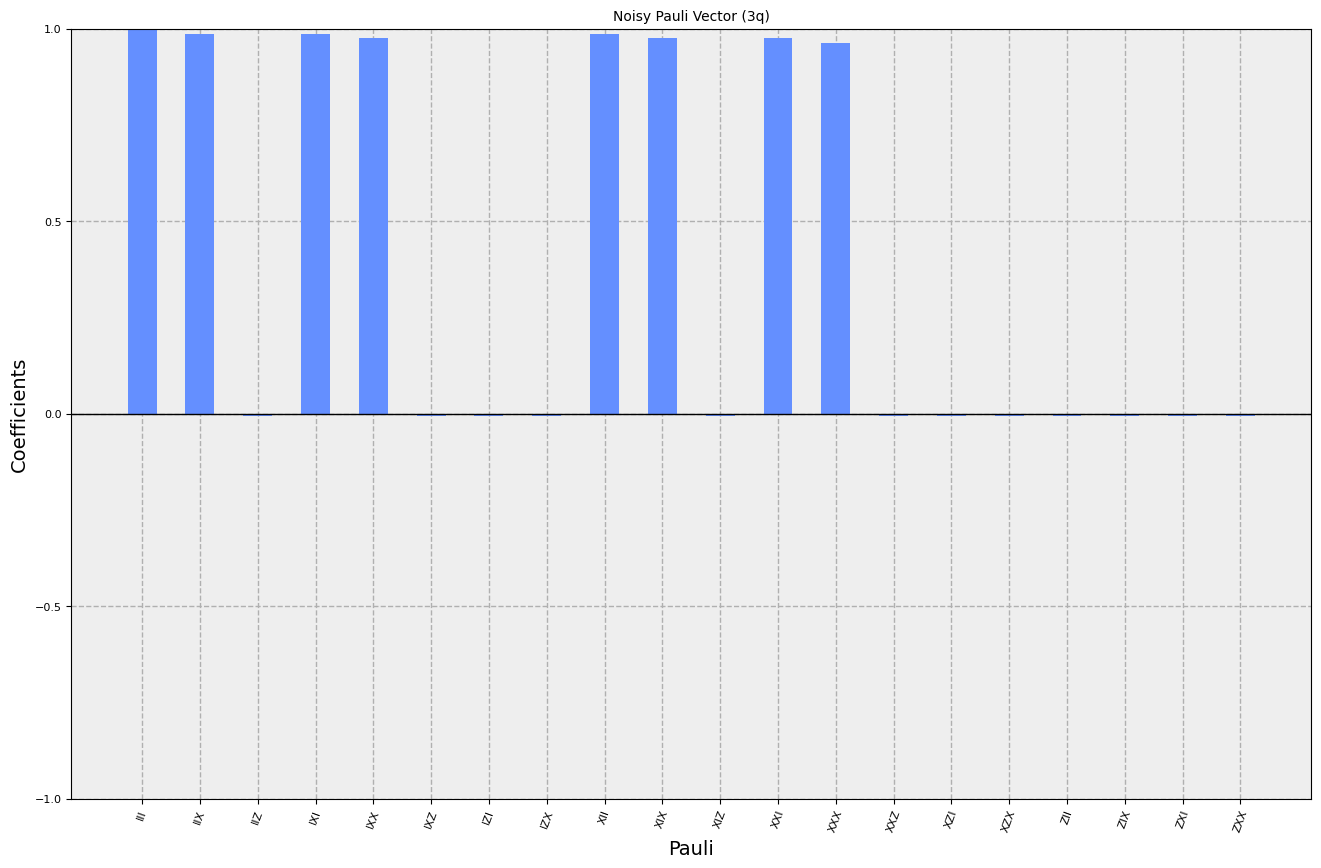
\includegraphics[width=0.75\linewidth]{pic/ch-Rice/PauliVector.png}
\vspace{\BeforeCaptionVSpace}
\caption{Pauli vector representation of the noisy quantum state. Shorter vectors indicate loss of coherence due to amplitude damping and depolarising noise.}
\label{fig:PauliVector}
\end{figure}

\subsection{Bloch Multivector}
The Bloch multivector plot represents the Bloch sphere components of each qubit individually. It helps visualise the influence of noise at the level of individual qubits, showing the deviation from the ideal pure state as shown in \textbf{Figure~\ref{fig:BlochMultivector}}.

\begin{figure}[htbp]
\centering
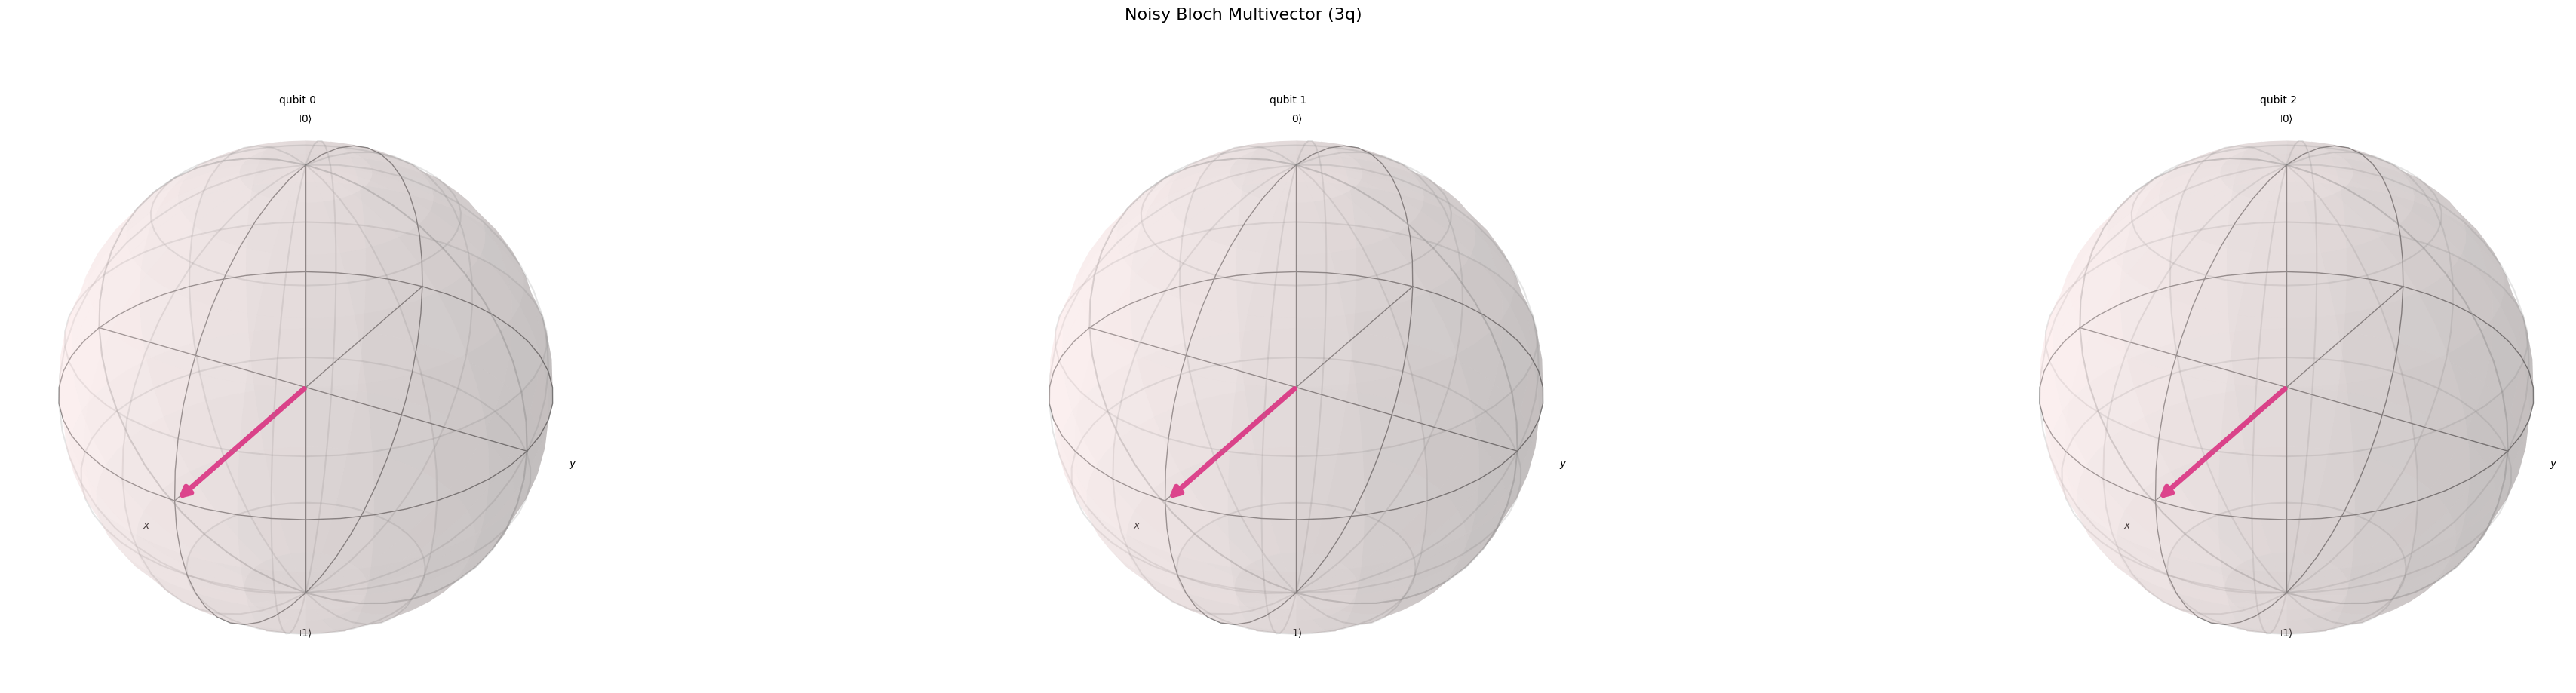
\includegraphics[width=0.75\linewidth]{pic/ch-Rice/MultiVector.png}
\vspace{\BeforeCaptionVSpace}
\caption{Bloch multivector visualisation showing each qubit’s Bloch representation. Deviation from pure state vectors indicates decoherence and noise effects.}
\label{fig:BlochMultivector}
\end{figure}

\subsection{Noisy Bitstring Count Histogram}
The resulting measurement distribution is visualised in \textbf{Figure~\ref{fig:NoisyHistogram}}. Ideally, in a noise-free simulation, each bitstring would occur with roughly equal frequency. However, the inclusion of depolarising and amplitude damping noise models introduces subtle biases into the sampling distribution. These imperfections reflect real-world quantum hardware limitations, and their impact is critical to evaluating the robustness of quantum-based latent encodings.

\begin{figure}[htbp]
\centering
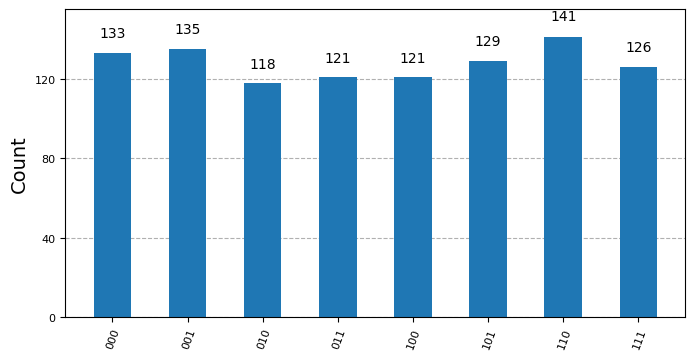
\includegraphics[width=0.70\linewidth]{pic/ch-Rice/HistoCount.png}
\vspace{\BeforeCaptionVSpace}
\caption{Measurement outcome histogram from quantum circuit under noise simulation. Bitstrings represent sampled latent vectors, exhibiting minor deviations due to quantum noise.}
\label{fig:NoisyHistogram}
\end{figure}

\section{Generator and Discriminator Training Dynamics}

\subsection{Discriminator Loss Dynamics}

The loss of the discriminator ($\mathcal{L}_D$) quantifies the degree of competence of the discriminator to distinguish between real and generated samples. Lower values indicate better discrimination performance, but excessively low loss may signal that the generator is underperforming or that the discriminator is overpowering the generator, potentially causing Mode Collapse.

As illustrated in \textbf{Figure~\ref{fig:DiscLoss}}, the Classical GAN exhibits a sharp and consistent increase in $\mathcal{L}_D$ as the number of samples seen increases from around 0.7M. This observation suggests a failure to maintain equilibrium with its generator. This is a common problem with Classical GAN, where the generator fails to keep up with the discriminator, leading to poor-quality outputs, inflated discriminator confidence, and mode collapse.

\begin{figure}[htbp]
\centering
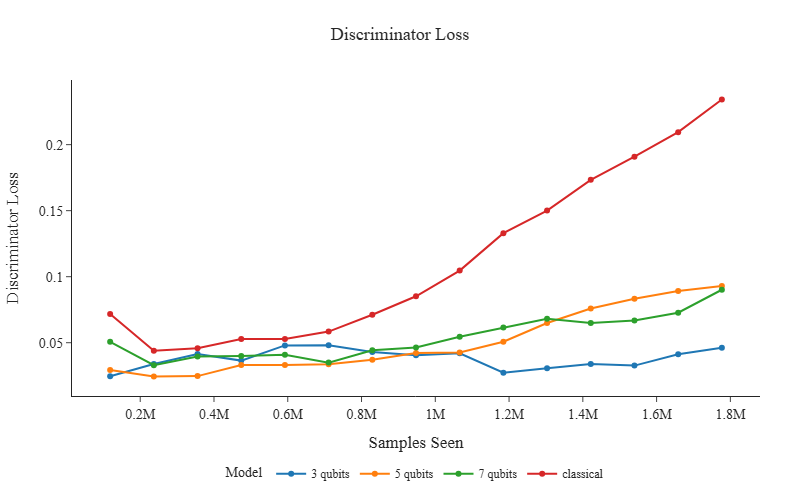
\includegraphics[width=0.75\linewidth]{pic/ch-Rice/Disc-Loss.png}
\vspace{\BeforeCaptionVSpace}
\caption{Discriminator loss trends ($\mathcal{L}_D$) across training for classical GAN and HQCGANs with 3, 5, and 7 qubits.}
\label{fig:DiscLoss}
\end{figure}

In contrast, all HQCGAN (3, 5, 7 qubits) demonstrate relatively stable $\mathcal{L}_D$, indicating a more sustained equilibrium adversarial training process. In particular, the 3 qubits HQCGAN (Blue Line) maintain the lowest and most stable $\mathcal{L}_D$ amongst the other HQCGANs. This implies that the generator was able to consistently fool the discriminator in training. The smooth gradient in these quantum-based losses suggests that quantum sampling may introduce latent diversity that supports more effective generator updates. 

These trends and observations empirically validate some theoretical advantages of the HQCGANs mentioned in Chapter~\ref{ch:review}. Specifically, the $\mathcal{L}_D$ trajectories of the HQCGAN reflect improved training stability and latent diversity compared to the Classical GAN.

\subsection{Generator Loss Dynamics}

The loss of the generator ($\mathcal{L}_G$) quantifies the degree of competence of the generator in generating samples similar to the training data. Lower values indicate better generator performance, but excessively low loss may signal that the discriminator is underperforming or that the generator is overpowering the discriminator, potentially causing mode collapse.

\begin{figure}[htbp]
\centering
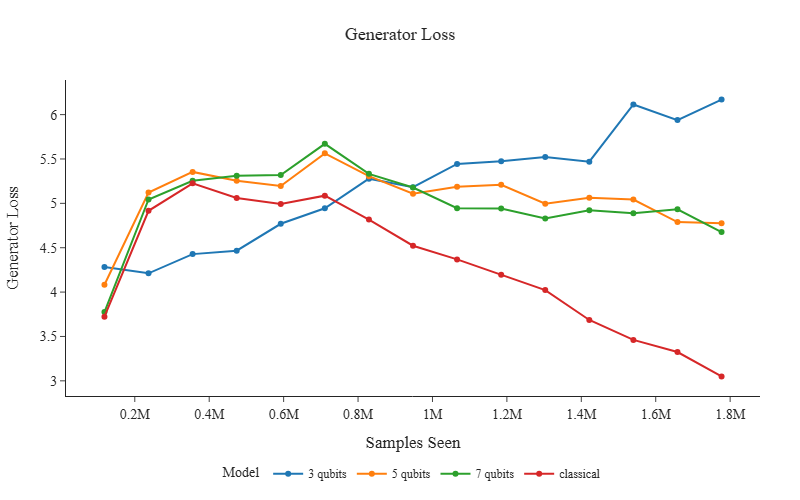
\includegraphics[width=0.75\linewidth]{pic/ch-Rice/Gen-Loss.png}
\vspace{\BeforeCaptionVSpace}
\caption{Generator loss trends across training for classical GAN and HQCGANs with 3, 5, and 7 qubits.}
\label{fig:GeneratorLoss}
\end{figure}

As illustrated in \textbf{Figure~\ref{fig:GeneratorLoss}}, the Classical GAN $\mathcal{L}_G$ steadily decreases when $N \approx 0.7M$, reaching values of $\mathcal{L}_G \approx 3$. Although this suggests that the generator is improving, the concurrent increase in $\mathcal{L}_D$ (from Chapter 3.3.1) suggests that this improvement may be artificial. The possibility of an overpowered generator dominating a weakening discriminator resulting in Mode Collapse cannot be ruled out in this scenario.

In contrast, all HQCGANs (3, 5, 7 qubits) exhibit stable $\mathcal{L}_G$ that oscillates within a narrow band where $4.5\leq\mathcal{L}_G\leq5.5$ throughout training. This oscillation is indicative of a healthy adversarial equilibrium. In particular, the 3-qubit HQCGAN display a slight upward gradient in $\mathcal{L}_G$ when $N \approx 1.4M$, potentially reflecting signs of under-fitting due to reduced latent dimensionality.

These dynamics observed reinforce the hypothesis that quantum-generated latent spaces introduce sufficient variability to prevent both premature convergence and over-fitting. The consistent $\mathcal{L}_G$ values suggest that quantum generators are constantly challenged by discriminators. Therefore, we maintain a productive adversarial training process in equilibrium without the occurrence of mode collapse.

\subsection{Combined Interpretation of Training Dynamics}

The adversarial equilibrium between the generator and the discriminator is critical for stable GAN training. The dual analysis of $\mathcal{L}_D$ and $\mathcal{L}_G$ in the classical GAN and HQCGAN reveals contrasting behavioural dynamics that underline the benefits of quantum-enhanced sampling.

In the classical GAN, the $\mathcal{L}_D$ increased significantly while $\mathcal{L}_G$ decreased steadily. This divergence suggests that the generator quickly exploited the fixed latent space and learnt to fool the discriminator too easily. Such a pattern is often seen as a symptom of mode collapse, where the generator output becomes overly repetitive, leading to poor diversity in generated samples despite a seemingly 'low' loss.

In contrast, the HQCGANs (3, 5, 7 qubits) demonstrated mutually stabilised loss profiles. $\mathcal{L}_D$ remained consistently low, indicating effective detection of generator outputs, while $\mathcal{L}_G$ maintained moderate values without sharp changes. This interplay implies a sustained adversarial challenge between the quantum generator and the classical discriminator, which encourages continuous improvements without mode collapse.

Moreover, the progressive increase in $\mathcal{L}_G$ with more qubits may reflect the growing complexity of the latent space. Higher qubit counts introduce richer and more entangled latent vectors, offering better diversity but also increasing the learning challenge for the generator.

In summary, the observed training dynamics suggests that HQCGAN not only solves the conventional problems faced by classical GANs, but also actively fulfils the theoretical advantages proposed in Chapter~\ref{ch:review}. Specifically, it fulfils the theoretical advantage of enhanced expressiveness and diversity from quantum noise.

\section{FID and KID Evaluation}

To evaluate the realism and diversity of the generated samples, two established metrics were tracked throughout training: \textbf{Fréchet Inception Distance (FID)} and \textbf{Kernel Inception Distance (KID)}. The formulas and rationale for these metrics were introduced in Chapter 3.1.

\subsection{Fréchet Inception Distance (FID)}

\textbf{Figure~\ref{fig:FID}} illustrates the progression of FID throughout the training of the classical GAN and HQCGAN. As expected, FID scores decreased consistently with the number of samples seen, indicating better alignment between the generated and true data distributions. Among the models, the classical GAN achieved the lowest overall FID scores, suggesting that it produced samples whose features most closely resembled those of the original dataset when evaluated using the Inception network.

\begin{figure}[htbp]
\centering
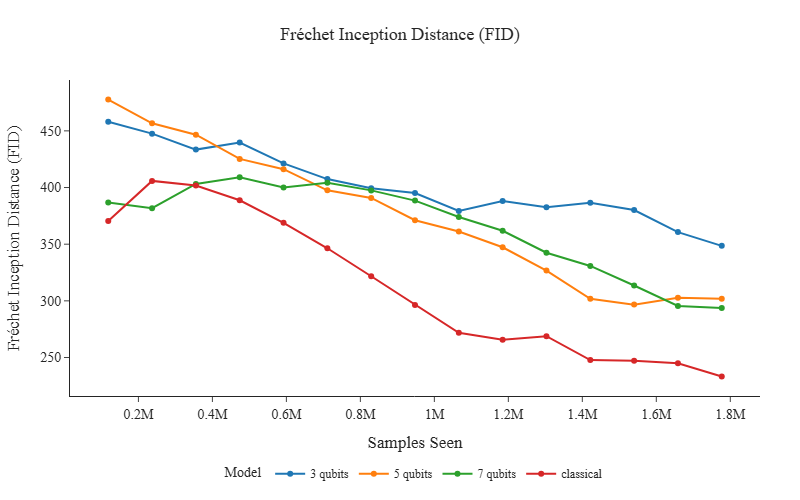
\includegraphics[width=0.7\linewidth]{pic/ch-Rice/FID.png}
\vspace{\BeforeCaptionVSpace}
\caption{Fréchet Inception Distance trends across training for classical GAN and HQCGANs with 3, 5, and 7 qubits.}
\label{fig:FID}
\end{figure}

Notably, 5-qubit and 7-qubit HQCGANs demonstrated competitive performance, particularly in the later stages of training. The 7-qubit model notably converged towards the classical GAN, indicating that greater quantum latent dimensionality may enhance sample fidelity. In contrast, the 3-qubit HQCGAN plateaued at a higher FID value where $N \approx 1$M, potentially due to the reduced representational capacity in the limited latent space dimensionality.
\newpage
\subsection{Kernel Inception Distance (KID)}

\textbf{Figure~\ref{fig:KID}} illustrates the Kernel Inception Distance (KID) curves over the training duration for the classical GAN and HQCGAN. KID, unlike FID, is based on the Maximum Mean Discrepancy (MMD) without the assumption of Gaussianity in the distribution of Inception features. This makes KID a more robust and unbiased measure, especially when the sample size is limited or the generative model produces outputs with diverse characteristics.

\begin{figure}[htbp]
\centering
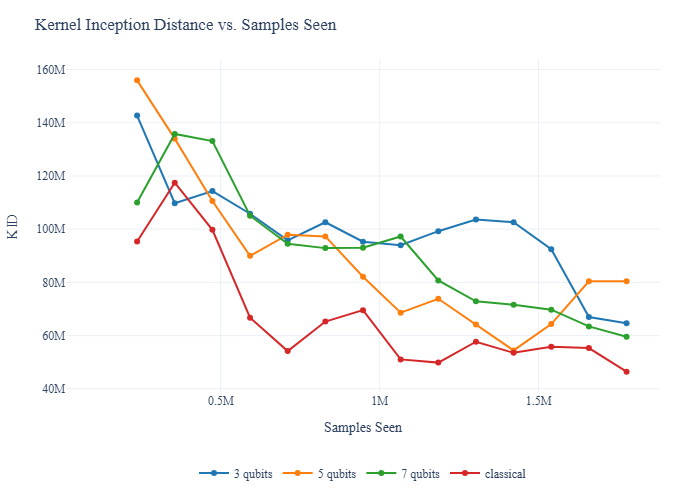
\includegraphics[width=0.7\linewidth]{pic/ch-Rice/KID.png}
\vspace{\BeforeCaptionVSpace}
\caption{Kernel Inception Distance trends across training for classical GAN and HQCGANs with 3, 5, and 7 qubits.}
\label{fig:KID}
\end{figure}

Across all models, KID scores generally decreased as training progressed, indicating improved alignment with the real data distribution. Although the classical GAN initially exhibited higher KID scores where $N \approx 0.4$M, it quickly outperformed all the HQCGANs. However, the 7-qubit HQCGAN consistently achieved competitive KID scores, especially beyond $N \approx 1.1$M sample seen. This suggests that increasing quantum latent dimensionality improves not only feature diversity but also robustness in distributional learning provided sufficient qubit is involved.

Given its impartial nature, KID should be treated as the primary metric to compare the performance of the GANs in this study. It captures subtle discrepancies that FID may overlook, particularly in models where Gaussian assumptions do not hold.

\subsection{Evaluation Metrics Discussion}

\textbf{Table~\ref{tab:metrics_evaluation}} illustrates the final evaluation metrics between the classical GAN and the HQCGAN (3, 5, 7 qubits). The sample seen ($N$) is consistent throughout all the GAN models. The final numerical values are derived from the trend curve in \textbf{Figure~\ref{fig:FID}} and \textbf{Figure~\ref{fig:KID}}.

\begin{table}[h]
  \centering
  \begin{tabular}{|l|c|c|c|c|}
    \hline
    Model & Classical & HQCGAN-3 & HQCGAN-5 & HQCGAN-7 \\ \hline
    Final FID & 201 & 330 & 307 & 294 \\ \hline
    Final KID (M) & 46.4 & 64.6 & 80.5 & 59.5 \\ \hline
  \end{tabular}
  \caption{Metrics Evaluation across Models.}
  \label{tab:metrics_evaluation}
\end{table}

With reference to Table~\ref{tab:metrics_evaluation}, the results further substantiate the hypothesis that increased quantum latent dimensionality improves the representational power of quantum generators. Although HQCGAN-3 struggled to match the classical GAN, most likely due to under-parameterisation, HQCGAN-7 closely matched the performance of the classical GAN’s performance, especially in the KID metric. The observed trends affirm the theoretical expectations of QGANs and HQCGANs, suggesting that quantum noise-injected latent sampling paired with classical discriminators can generate diverse and distribution-consistent data, provided that the quantum circuit has sufficient capacity.

\section{Efficiency and Scalability}

In addition to evaluating generative capabilities through quantitative metrics such as FID and KID, it is equally crucial to evaluate the efficiency and scalability of HQCGANs due to the theoretical promises of more efficient training duration. These aspects become especially pertinent in the context of quantum-based models, where access to quantum hardware is limited, and simulation time on classical back-ends can be substantial.

\begin{table}[h]
  \centering
  \begin{tabular}{|l|c|c|c|c|}
    \hline
    Model & Classical & HQCGAN-3 & HQCGAN-5 & HQCGAN-7 \\ \hline
    Qubits Used & 0 & 3 & 5 & 7 \\ \hline
    Latent Dim & 100 & 3 & 5 & 7 \\ \hline
    Avg. Time per 1M Sample (s) & 186.51 & 203.71 & 203.98 & 212.00 \\ \hline
    Total Quantum Shots & 0 & 23808 & 23808 & 23808 \\ \hline
  \end{tabular}
  \caption{Efficiency Comparison across Models.}
  \label{tab:efficiency_comparison}
\end{table}
\newpage
\textbf{Table~\ref{tab:efficiency_comparison}} presents the efficiency metrics across all GAN models. As expected, the classical GAN exhibits the lowest average run-time per million samples, due to its purely neural nature without any quantum simulation overhead. However, all HQCGAN models maintain comparable runtimes, with only a slight increase observed as the number of qubits rises from 3 to 7. This suggests that quantum latent sampling scales efficiently in simulation and may remain feasible on near-term quantum hardware.

Although classical GANs are faster, HQCGANs demonstrate respectable training efficiency and show promise in representing complex distributions with significantly reduced latent dimensionality. This highlights their potential as compressed generative architectures with competitive performance-to-cost trade-offs. The efficiency may also deviate from the theoretical lens due to the lack of quantum hardware and usage of quantum simulation.

\section{Summary of Findings}

This chapter explored the implementation and comparative evaluation of classical GANs and HQCGANs on a binary variant of the MNIST dataset. Three HQCGAN configurations were tested, with 3, 5, and 7 qubits serving as quantum latent dimensions. A consistent generator and discriminator architecture was used across all models, with quantum circuits generating latent vectors subject to simulated device-level noise.

Visual inspection of the quantum circuit output confirmed high-entropy, non-degenerate sampling across all qubit variants. Despite reduced latent dimensionality, the HQCGANs—particularly the 7-qubit model—demonstrated competitive training dynamics and generative capability. The discriminator and generator loss curves showed convergence behaviours similar to the classical GAN.

Evaluation metrics further validated these trends. The \textbf{Fréchet Inception Distance (FID)} and \textbf{Kernel Inception Distance (KID)} steadily improved with training for all models. While the classical GAN attained the lowest FID score, the HQCGAN with 7 qubits achieved comparable results in later epochs.

Efficiency analysis showed that the usage of quantum shots remained fixed according to the HQCGAN model, regardless of the complexity of the data. Training time scaled linearly with the number of qubits, with HQCGAN-3 offering the fastest runtime amongst the HQCGANs. In general, the findings generally support the hypothesis that HQCGANs offer a viable generative alternative within the constraints of the \textbf{Noisy Intermediate-Scale Quantum (NISQ)} capabilities, balancing quantum expressiveness with classical efficiency.
